
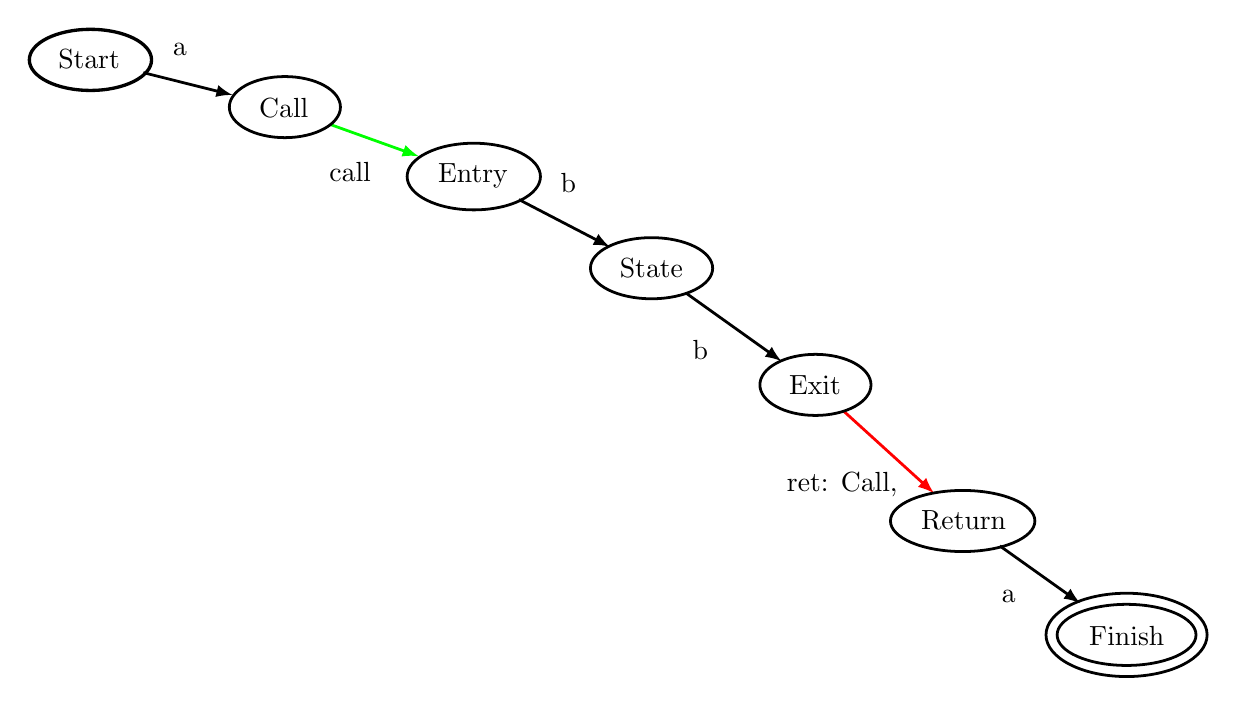
\begin{tikzpicture}[>=latex,line join=bevel,]
  \pgfsetlinewidth{1bp}
%%
\pgfsetcolor{black}
  % Edge: Call -> Entry
  \pgfsetcolor{green}
  \draw [->] (110.44bp,199.71bp) .. controls (117.12bp,197.31bp) and (125bp,194.48bp)  .. (142.17bp,188.32bp);
  \definecolor{strokecol}{rgb}{0.0,0.0,0.0};
  \pgfsetstrokecolor{strokecol}
  \draw (117.5bp,182.74bp) node {call};
  % Edge: Entry -> State
  \draw [->] (178.25bp,172.72bp) .. controls (185.43bp,168.98bp) and (193.99bp,164.53bp)  .. (210.99bp,155.7bp);
  \draw (196.06bp,178.58bp) node {b};
  % Edge: Start -> Call
  \draw [->] (43.027bp,218.41bp) .. controls (49.935bp,216.68bp) and (57.85bp,214.7bp)  .. (75.143bp,210.37bp);
  \draw (56.182bp,226.62bp) node {a};
  % Edge: Return -> Finish
  \draw [->] (351.38bp,48.031bp) .. controls (357.36bp,43.768bp) and (364.68bp,38.56bp)  .. (380.28bp,27.456bp);
  \draw (354.53bp,29.801bp) node {a};
  % Edge: Exit -> Return
  \pgfsetcolor{red}
  \draw [->] (295.15bp,96.552bp) .. controls (302.24bp,90.112bp) and (311.84bp,81.388bp)  .. (327.69bp,66.987bp);
  \definecolor{strokecol}{rgb}{0.0,0.0,0.0};
  \pgfsetstrokecolor{strokecol}
  \draw (294.67bp,70.177bp) node {ret: Call, };
  % Edge: State -> Exit
  \draw [->] (238.43bp,139.03bp) .. controls (246.02bp,133.61bp) and (255.91bp,126.56bp)  .. (272.77bp,114.53bp);
  \draw (243.51bp,118.69bp) node {b};
  % Node: Finish
\begin{scope}
  \definecolor{strokecol}{rgb}{0.0,0.0,0.0};
  \pgfsetstrokecolor{strokecol}
  \draw (397bp,16bp) ellipse (25bp and 11bp);
  \draw (397bp,16bp) ellipse (29bp and 15bp);
  \draw (397.08bp,15.5bp) node {Finish};
\end{scope}
  % Node: Return
\begin{scope}
  \definecolor{strokecol}{rgb}{0.0,0.0,0.0};
  \pgfsetstrokecolor{strokecol}
  \draw (338bp,57bp) ellipse (26bp and 11bp);
  \draw (338.34bp,57.309bp) node {Return};
\end{scope}
  % Node: Start
\begin{scope}
  \definecolor{strokecol}{rgb}{0.0,0.0,0.0};
  \pgfsetstrokecolor{strokecol}
  \draw [very thick] (24bp,223bp) ellipse (22bp and 11bp);
  \draw (23.5bp,223.3bp) node {Start};
\end{scope}
  % Node: State
\begin{scope}
  \definecolor{strokecol}{rgb}{0.0,0.0,0.0};
  \pgfsetstrokecolor{strokecol}
  \draw (226bp,148bp) ellipse (22bp and 11bp);
  \draw (225.94bp,147.93bp) node {State};
\end{scope}
  % Node: Call
\begin{scope}
  \definecolor{strokecol}{rgb}{0.0,0.0,0.0};
  \pgfsetstrokecolor{strokecol}
  \draw (94bp,206bp) ellipse (20bp and 11bp);
  \draw (93.601bp,205.75bp) node {Call};
\end{scope}
  % Node: Entry
\begin{scope}
  \definecolor{strokecol}{rgb}{0.0,0.0,0.0};
  \pgfsetstrokecolor{strokecol}
  \draw (162bp,181bp) ellipse (24bp and 12bp);
  \draw (161.7bp,181.31bp) node {Entry};
\end{scope}
  % Node: Exit
\begin{scope}
  \definecolor{strokecol}{rgb}{0.0,0.0,0.0};
  \pgfsetstrokecolor{strokecol}
  \draw (285bp,106bp) ellipse (20bp and 11bp);
  \draw (284.84bp,105.93bp) node {Exit};
\end{scope}
%
\end{tikzpicture}
